\section{Salze}

\subsection{Aufbau}
Salzartige Stoffe bestehen aus Ionen (el. geladene Atome oder Moleküle). Zwischen den Ionen herrschen ungerichtete elektrostatische Kräfte.\\ Kationen $\Rightarrow$ oft Metallionen\\Anionen $\Rightarrow$ \emph{immer} Nichtmetallionen \\
Ionische Bindung: Elektrostatische Wechselwirkungen zwischen allen Kationen und Anionen. $F = \frac{1}{4 \pi \epsilon_0} \cdot \frac{Q_1 + Q_2}{d^2}$ \\
Kristalline Stoffe, oft in dichtester Kugelpackung angeordnet, (abhängig von Ionengrösse und Ionenverhältnis) z.B. NaCl-Typ:
\begin{figure}[h!]
	\centering
	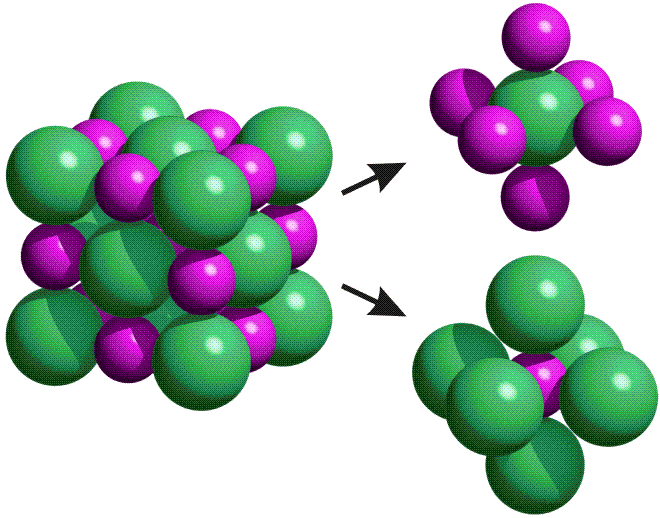
\includegraphics[width=0.4\linewidth]{images/5_Elementarzelle_NaCl.png}
\end{figure}

\subsection{Salzformeln}
Salzformeln sind Verhältnisformeln.
\begin{enumerate}[nolistsep]
	\item Die Ladungen der Ionen ergeben sich aus der Edelgasregel $\Rightarrow$ PSE: Hauptgruppe (HG) 1 bis 3 wollen $e^-$ abgeben, dh. Ionenladung = + HGNr.; HG 5 bis 7 wollen $e^-$ aufnehmen, dh. Ionenladung = - (8 - HGNr.)\\ 
	Bsp: Na $\Rightarrow$ Na$^+$, Al $\Rightarrow$ Al$^{3+}$ (möchte 3 e$^-$ abgeben), Cl $\Rightarrow$ Cl$^-$, O $\Rightarrow$ Na$^{2-}$ (möchte 2 e$^-$ aufnehmen)
	\item Salze sind insgesamt neutral. \\
	Bsp: Na $\Rightarrow$ Na$^+$: Cl$^-$ = 1:1  $\Rightarrow$  NaCl,\\
	Al$^{3+}$: O$^{2-}$ = 2:3 $\Rightarrow$ Al$_2$O$_3$
\end{enumerate}

\subsection{Nomenklatur}
Name Kation + (griech./lat.) Name Anion + \emph{-id} \\
Bei Übergangsmetallen: Kationenladung als römische Ziffer. 

\subsection{Gitterenergie}
$E_G$: Energie, um ein Salz in seine freien Ionen zu zerlegen (bzw. umgekehrt). Wird vor allem durch die Coulombkraft bestimmt. Wird umso grösser: je grösser die Ionenladungen und je kleiner die Ionenradien (Atomradien nehmen innerhalb einer Gruppe des PSE von oben nach unten zu und innerhalb einer Periode von links nach rechts ab) sind.

\subsection{Eigenschaften}
\subsubsection{Sprödigkeit}
Die Sprödigkeit sagt aus, wie stark sich ein Stoff verformen lässt bis er bricht. Bei Verformung eines Salzes müssen die Kationen- und Anionenebenen (durch eine externe Kraft) gegeneinander verschoben werden (so geraten Kationen neben Kationen und Anionen neben Anionen) $\Rightarrow$ Abstossung $\Rightarrow$ Bruch des Salzes

\subsubsection{Schmelz- und Siedepunkt}
Aufgrund der Coulumb-Kräfte, weisen Salze hohe Schmelz- (in der Regel über 400$^\circ$C) und Siedepkt. auf $\Rightarrow$ Sie sind somit schwerflüchtige (hoher Siedepkt.) Verbindungen. Schmelz(mp)- und Siedepkt.(bp) kann mit Hilfe der Gitterenergie abgeschätzt werden. D.h. je höher die Gitterenergie, desto höher der Schmelz- bzw. Siedepkt. 

\subsubsection{Elektrische Leitfähigkeit}
Feste Salze: keine elektrische Leitfähigkeit (el. Isolatoren); Salzschmelzen und Salzlösungen: gute Leitfähigkeit.\\
Die Leitfähigkeit einer Salzlösung ist abhängig von 3 Faktoren: Anionen- und Kationenkonzentrationen, Ladungszahlen der Anionen und Kationen, Beweglichkeiten der Anionen und Kationen

\subsubsection{Löslichkeit}
\begin{figure}[h!]
	\centering
	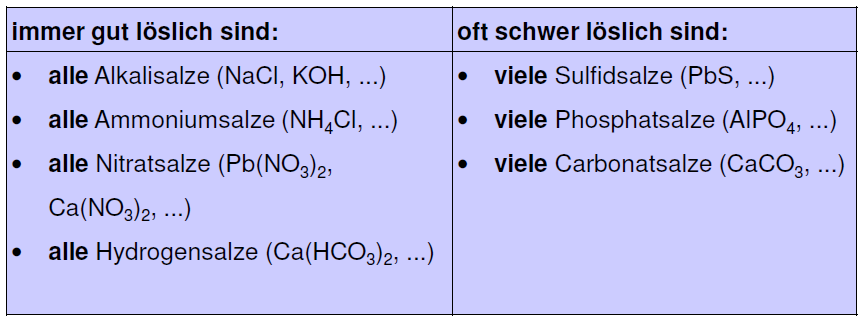
\includegraphics[width=0.9\linewidth]{images/5_Tabelle_Loeslichkeit.png}
\end{figure}
Sobald ein Salz mit einer polaren Flüssigkeit (z.B. Wasser) in Berührung kommt, ziehen die Ionen an der Oberfläche des Salzes die Dipolmoleküle an: Die negativen Pole ($\delta-$) der Dipolmoleküle werden von den Kationen, die positiven Pole ($\delta+$) von den Anionen angezogen. Temperaturschwingungen begünstigen das Eindringen von Dipolmolekülen zwischen Anionen und Kationen, was eine Schwächung der elektrostatischen Kräfte zur Folge hat. Die einzelnen Ionen können somit vollständig von Dipolmolekülen umhüllt werden und sich vom Salzkristall ablösen.

Schreibweise: $NaCl_{(s)} \, \rightarrow \, Na^+_{(aq)} + Cl^-_{(aq)}$